What does our model capture?
What are the functionalities of our system?
What's necessary in a model?
Which formalism to use? (reason for the choice)

\section{Universally Composable Framework}

\section{Protocol Overview}
The protocol can be described in four parts, the extended TrustChain datastructure, 
the consensus protocol, the transaction protocol and finally the validation protocol.
We first describe how the protocols work individually and then explain how they fit together.

\subsection{Extended TrustChain}
Extended TrustChain naturally builds on top of TrustChain, thus we first describe the standard TrustChain.
Our description has minor differences compared to the description in~\cite{trustchain}.
This is to help with the description of the extended TrustChain.
However, the two descriptions are functionally the same.

\subsubsection*{Standard TrustChain}
In TrustChain, every node has their ``personal'' chain. 
Initially, the chain only contains a genesis block.
When a node wishes to add a new transaction (TX), a new TX block is generated and is appended to the chain.
A TX block must have a valid hash pointer pointing to the previous block
and a reference\footnote{TODO This is the difference?} to its \emph{pair}.
Suppose Alice made a transaction with Bob, then both parties must create a TX block to acknowledge that the transaction took place.
The pair of Alice's TX block is the corresponding TX on Bob's chain and vice versa.
An example of 3 nodes is shown in \Cref{fig:trustchain-bad}.

\begin{figure}
    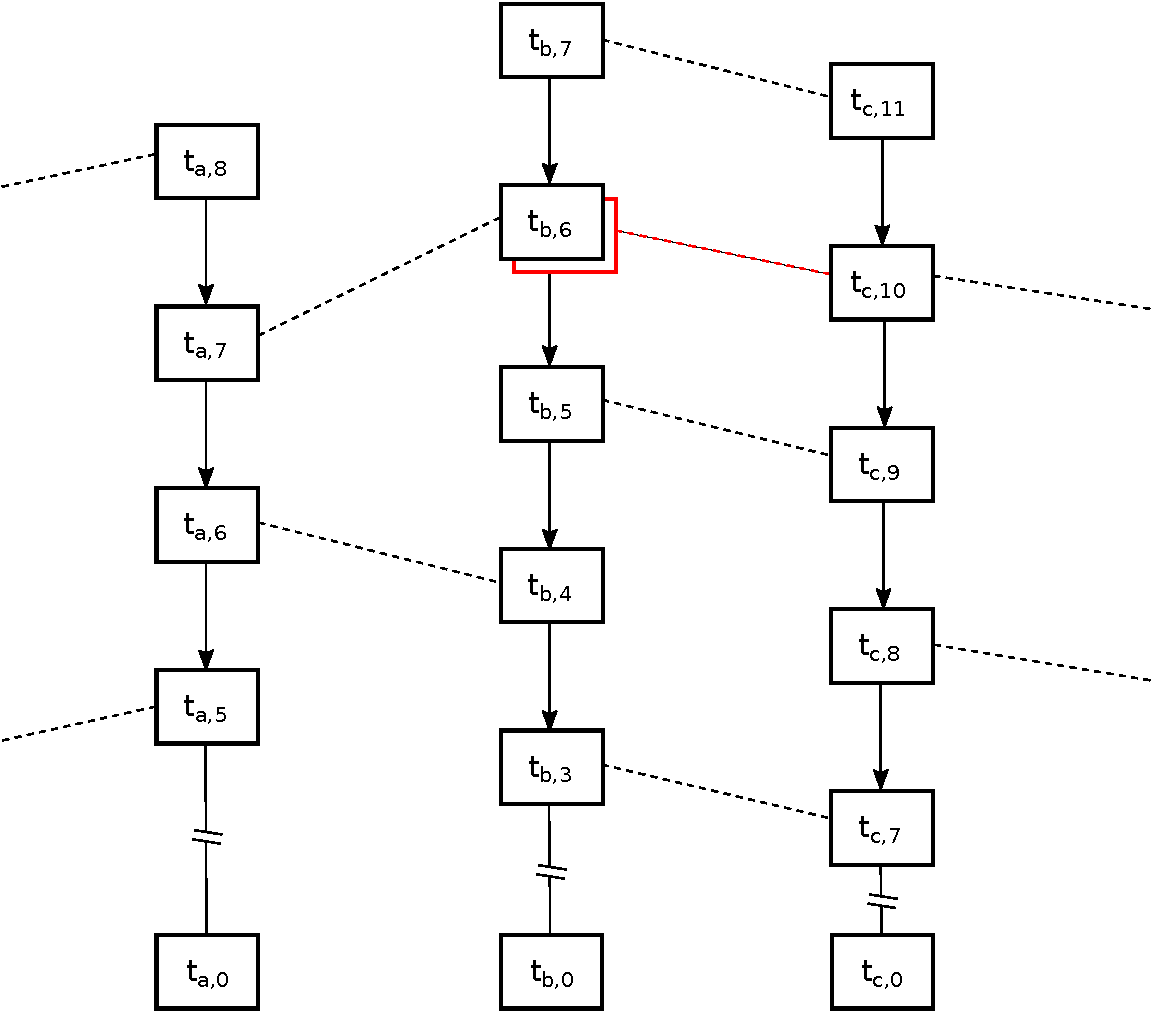
\includegraphics[width=0.8\textwidth]{trustchain-bad}
    \centering
    \caption{Every block is denoted by $t_{i,j}$, where $i$ is the node ID and $j$ is the sequence number of the block.
    Thus we have three nodes and three corresponding chains in this example.
    The arrows represent hash pointers and the dotted lines represent references.
    The blocks at the ends of one dotted line are pairs of each other.
    The red block after $t_{b, 5}$ indicate a fork.}
    \label{fig:trustchain-bad}
\end{figure}

If every node follows the rules of TrustChain and we only consider hash pointers,
then the chain effectively forms a singly linked list.
However, if a node violates the rules, then a \emph{fork} may happen.
That is, there may be more than one TX block with a hash pointer pointing back to the same block.
In \Cref{fig:trustchain-bad}, node $b$ (in the middle chain) created two TX blocks that both point to $t_{b, 5}$.
If this is a ledger system it can be seen as a double spend, where the currency accumulated up until $t_{b, 5}$ are spent twice.

\subsubsection*{Extended TrustChain}
We are now ready to explain the extended TrustChain, which we abbreviate to ETC.
In ETC, we introduce a new type of block, namely checkpoint (CP) block.
In contract to TX blocks, CP blocks do not store transactions or contain references.
They capture the state of the chain and the state of the whole system.
In particular, the state of the chain is captured with a hash pointer.
The state of the whole system is captured in the content of the CP block,
namely as a digest of the latest \emph{consensus result} which we explain in \Cref{sec:overview-cons}.
A visual representation is shown in \Cref{fig:trustchain-bad-cp}.

\begin{figure}
    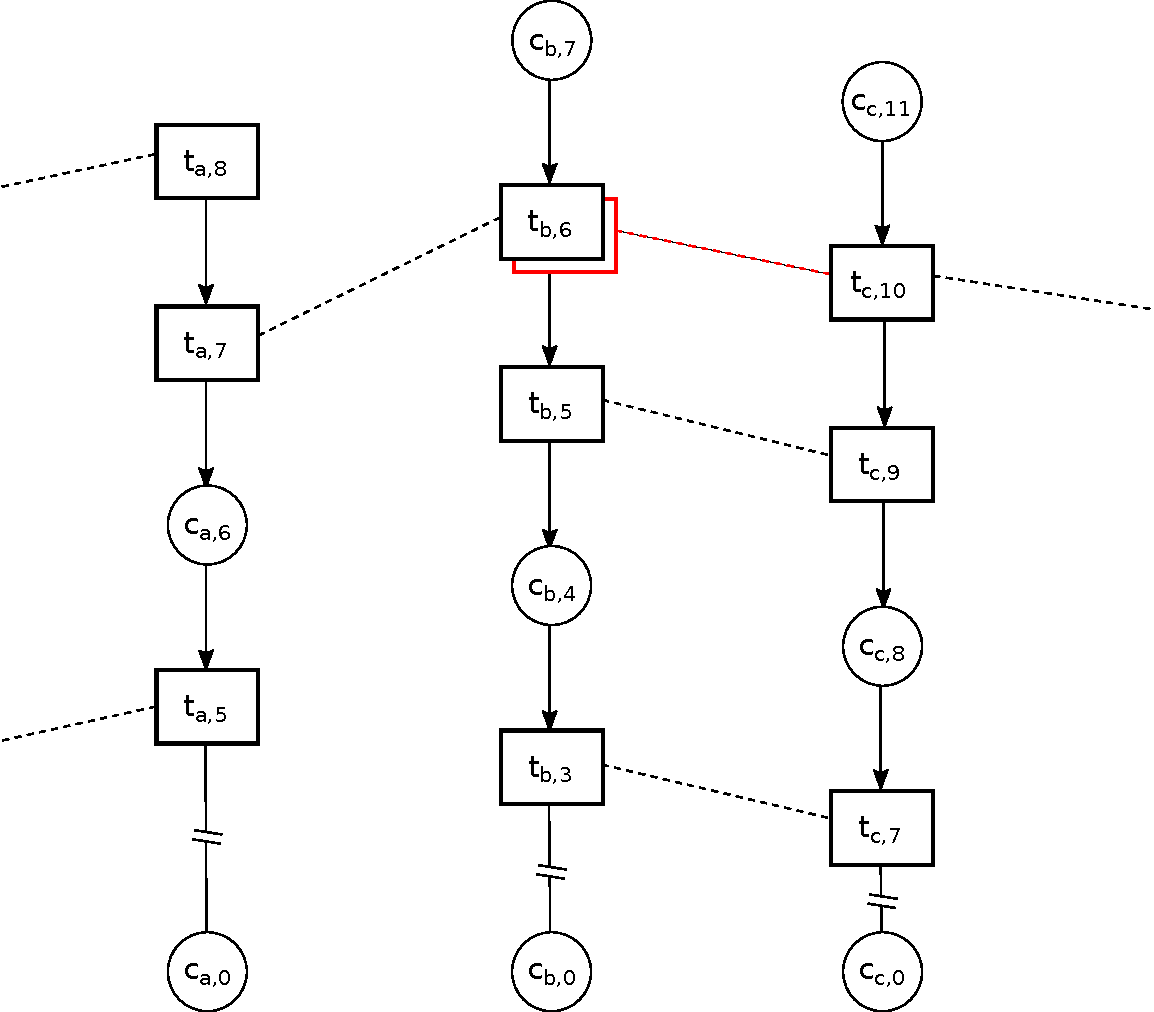
\includegraphics[width=0.8\textwidth]{trustchain-bad-cp}
    \centering
    \caption{TODO}
    \label{fig:trustchain-bad-cp}
\end{figure}

\subsection{Consensus Protocol}\label{sec:overview-cons}
Before describing our consensus protocol, we take a brief detour to explain Byzantine consensus,
which is a fundamental building block of our consensus protocol.

\subsubsection*{Byzantine consensus}
Byzantine consensus is also known as \emph{atomic broadcast}.
Roughly speaking, atomic broadcast need to satisfy the following properties.
\begin{enumerate}
\item TODO
\end{enumerate}
We stress that Byzantine consensus is not the same as Byzantine agreement or the Byzantine general's problem.
Byzantine agreement is TODO

The literature on Byzantine consensus and atomic broadcast is rich, some noteable ones include TODO.
Thus in the ETC consensus protocol, we assume there exist an "off-the-shelf" Byzantine consensus algorithm which we can use
(in our implementation we use HoneyBadgerBFT and motivate our choice in TODO).

\subsubsection{ETC consensus protocol} 
We explain the consensus protocol using the example in 

\subsection{Transaction Protocol}

\subsection{Validation Protocol}

\subsection{Putting Everything Together}

\section{Extended TrustChain Protocol}

\section{Protocol Extensions}